\documentclass[tikz,border=10pt]{standalone}
\usepackage{tikz}
\begin{document}
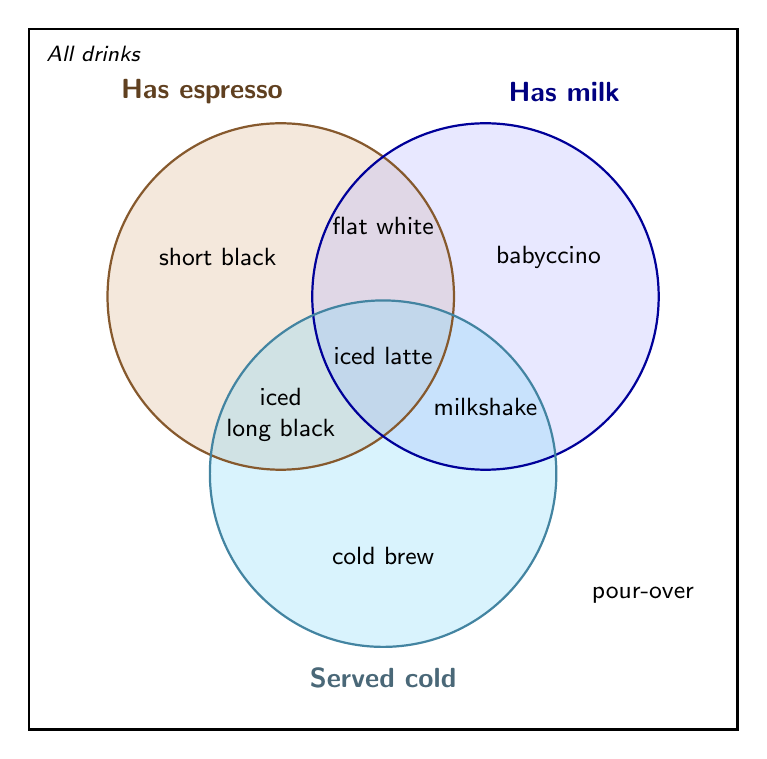
\begin{tikzpicture}[font=\sffamily\small]
\def\r{2.2}
\coordinate (E) at (0,0);
\coordinate (M) at (2.6,0);
\coordinate (C) at (1.3,-2.25);
\draw[thick] (-3.2,-5.5) rectangle (5.8,3.4);
\node[anchor=north west,font=\sffamily\footnotesize\itshape] at (-3.1,3.3) {All drinks};
\fill[brown!60,opacity=.3] (E) circle (\r);
\fill[blue!30,opacity=.3] (M) circle (\r);
\fill[cyan!50,opacity=.3] (C) circle (\r);
\draw[thick,brown!70!black] (E) circle (\r);
\draw[thick,blue!60!black] (M) circle (\r);
\draw[thick,cyan!60!black] (C) circle (\r);
\node[font=\sffamily\bfseries,brown!50!black] at (-1.0,2.6) {Has espresso};
\node[font=\sffamily\bfseries,blue!50!black] at (3.6,2.6) {Has milk};
\node[font=\sffamily\bfseries,cyan!40!black] at (1.3,-4.85) {Served cold};
% regions
\node at (-0.8,0.5) {short black};
\node at (3.4,0.5) {babyccino};
\node at (1.3,-3.3) {cold brew};
\node at (1.3,0.9) {flat white};
\node[align=center] at (0.0,-1.5) {iced\\long black};
\node at (2.6,-1.4) {milkshake};
\node at (1.3,-0.75) {iced latte};
\node at (4.6,-3.8) {pour-over};
\end{tikzpicture}
\end{document}
